\section{Edge Detection}

Edges are widely used in computer vision, they contain rich information about texture 
and geometry, for this reason edges are features that are useful for several tasks, 
such as object recognition, object tracking, etc.


The Sobel filter is a well known edge detector. To apply this filter is necessary to 
convolve the image with two $3\times3$ matrices, to find intensity changes in vertical and 
horizontal directions:

\begin{center}

\includegraphics[scale=0.35]{images/sobel}
\end{center}

Then both results are merged using the bellow expression and a threshold is used to filter out non interest areas:

\begin{equation}
G = \sqrt{G_x^2+ G_y^2}\ .
\label{eq:sobelGrad}
\end{equation}

This filter was used to obtain a representative set of points, avoiding that walls and another 
plain surfaces containing a huge amount of data, lead to an incorrect alignment.
There are more advanced edge filtering techniques, such as the Canny edge filter, but it involves 
a larger set of convolutions and operations. Since we don't need a high accuracy edge detection, the Sobel 
filter is enough to reduce the set of points used in the alignment process. 

The filter was applied directly into a grayscale representation of the original RGB image. Obtaining a binary image 
that contains edges representing geometrical and visual changes in the scene. 
This image can be used along with the depth map to reduce the point cloud size. Because dataset RGB and depth map images are 
calibrated, a pixel $(x,y)$ in the RGB image corresponds to the same $(x,y)$ location in the depth map. Thus, we can perform filtering 
in the RGB image and then modify depth map using the same coordinates. The binary image obtained from Sobel filter, was used 
to reject all points not corresponding
to these edges in the depth map. 

Edge filtering was applied
to the image instead of the depth map. Because using this approach it is possible to find correspondences between rich textured 
surfaces, even if they don't exhibit local geometrical changes.

The applied threshold for the Sobel filter was low, in order to have thicker edges. Because if too few points pass the filter, important information 
could be lost, difficulting a correct alignment.


\begin{figure}
\begin{center}
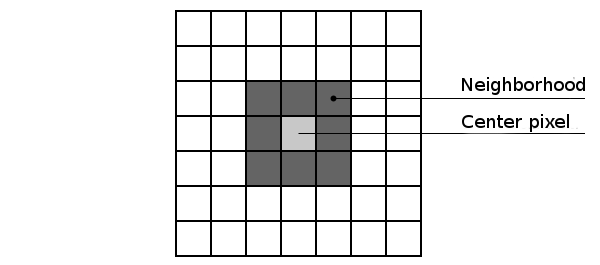
\includegraphics[scale=0.4]{images/vecindario}
\end{center}
\caption{pixel neighborhood.}
\label{fig:neighbor}
\end{figure}

In combination with a low threshold used in the Sobel filter applied to the grayscale image, all points of the neighborhood of the corresponding depth map pixels passing the Sobel filter were added. 
The neighborhood is defined as shown in figure ~\ref{fig:neighbor}. The purpose of this is to have enough points even if few points
 pass Sobel filter.

This filter is applied to both, source and target captures. Making this, it is possible to apply a very useful filtering: remove 
from both point clouds all the points that are not in common. For this, the rotation and translation 
of the source Sobel filtered 2D image that minimizes the distance between the closest pixels of the Sobel filtered target 2D image is found and 
then applied to each pixel of the source depth map, 
allowing to apply an AND operation as follows: if transformed source depth map pixel has a correspondent pixel in the target depth map and 
the euclidean distance (in the 3D space) is less than a threshold, maintain both pixels (of source and target depth maps), in other case reject them. 

 As result, we work with two point clouds that have a huge amount of overlapping points, improving the alignment 
result. The AND ensures that both depth map pixels (from source and target depth maps) are present in the two point clouds (at least from viewing 
perspective) and the distance filtering filters out pairs of points that pass the AND filter, but are too far in the euclidean space.

\begin{figure}[H]
\begin{center}
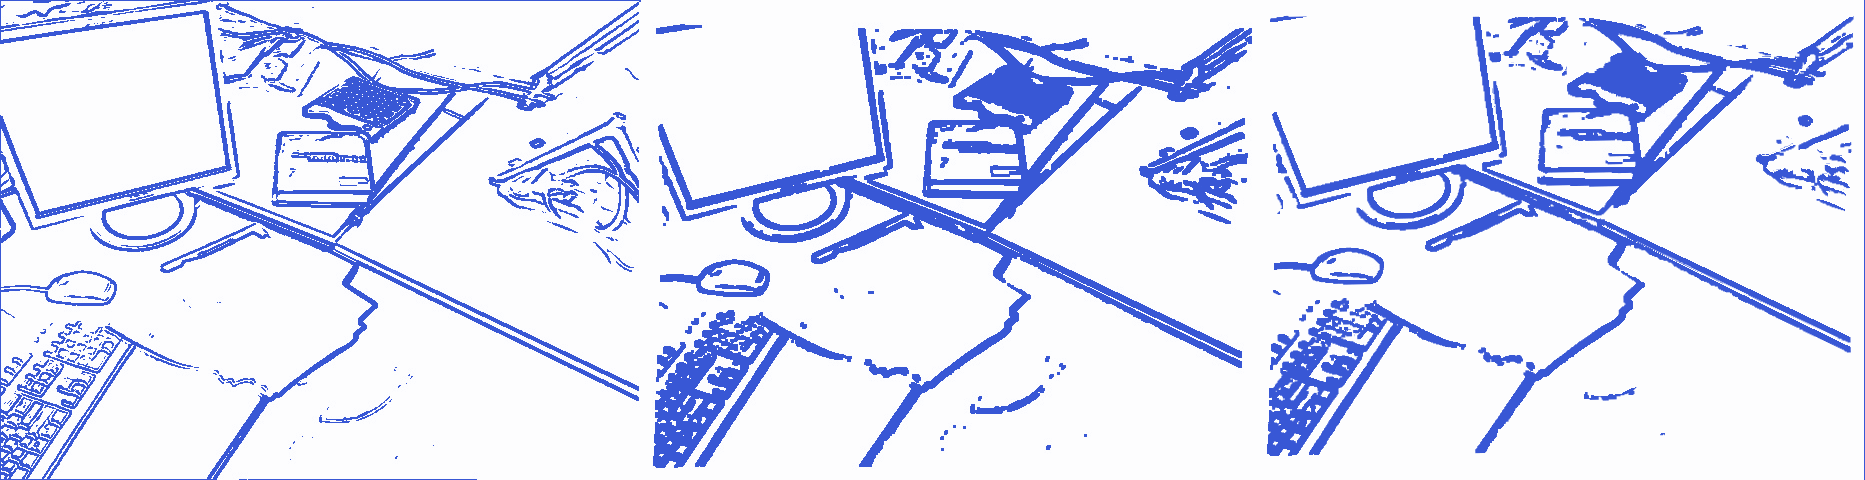
\includegraphics[scale=0.2]{images/borders_steps.png}
\caption{Left: image after applying sobel filter. Middle: image after adding depth map neighborhood points. Right: image after
applying AND operation and distance filtering between the two consecutive point clouds.}
\end{center}
\end{figure}


\begin{figure}[H]
\begin{center}
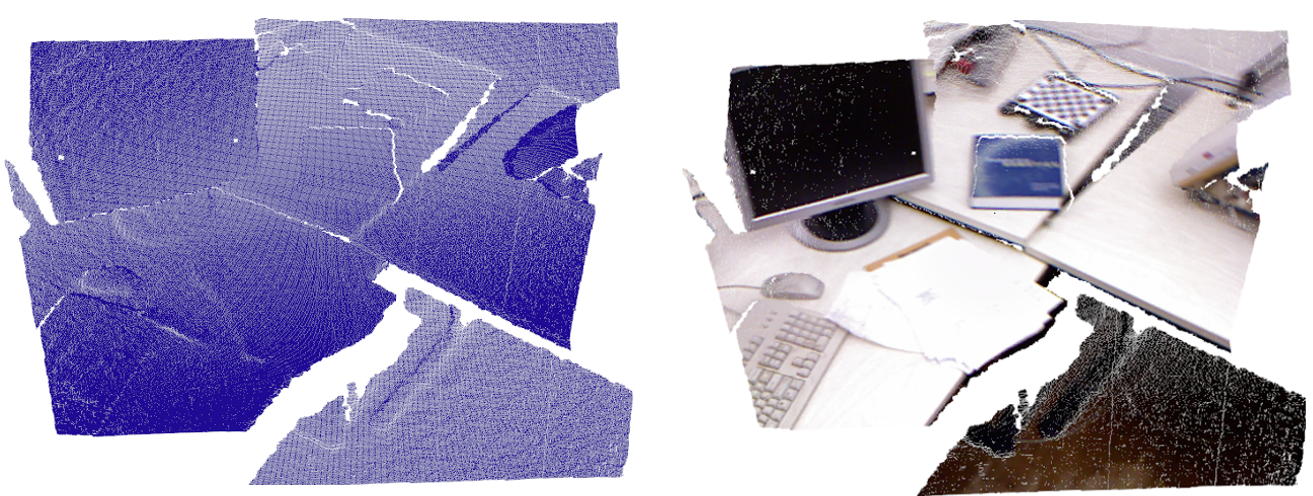
\includegraphics[scale=0.3]{images/borders_orig.png}
\caption{One of the point clouds before applying filter.}
\end{center}
\end{figure}


\begin{figure}[H]
\begin{center}
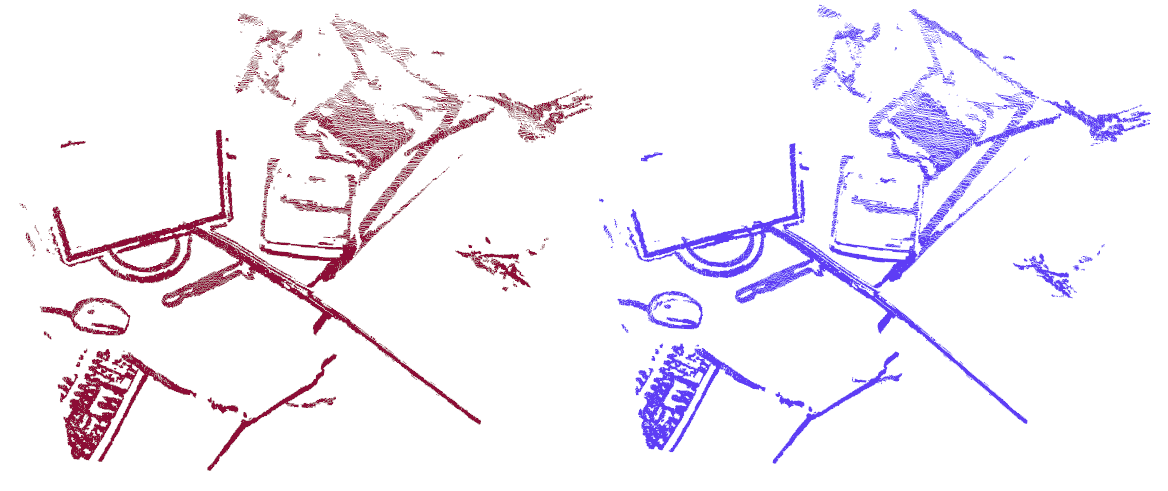
\includegraphics[scale=0.3]{images/borders_consec.png}
\caption{Two consecutive point clouds  after edge filtering.}
\end{center}
\end{figure}

\begin{figure}[H]
\begin{center}
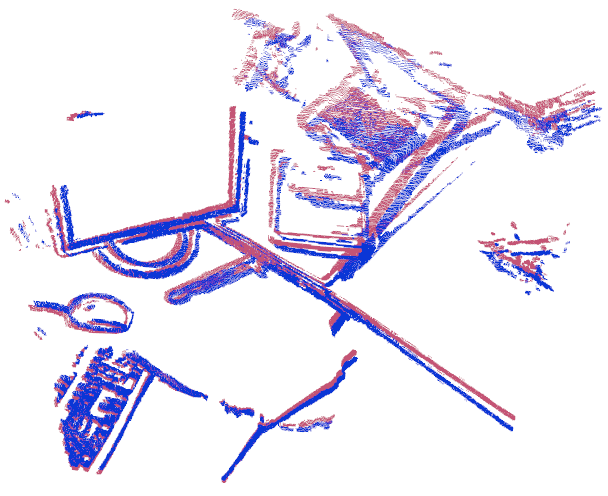
\includegraphics[scale=0.3]{images/borders_both.png}
\caption{Both filtered point clouds shown in the same coordinate system.}
\end{center}
\end{figure}


\begin{algorithm}[H]
\caption{Edge filtering algorithm}
\label{alg:edges}
\begin{algorithmic}[1]
\State grayImageSrc = RGBtoGray(srcImage)
\State grayImageTgt = RGBtoGray(tgtImage)
\State sobelSrc = sobelFilter(grayImageSrc)
\State sobelTgt = sobelFilter(grayImageTgt)
\State T = FindRigidTransformation(sobelSrc,sobelTgt)
\ForAll {x in [0-640] and y in [0-320]} 
\If {$sobelSrc(x,y) > 0$ AND $DepthMapSrc(x,y) > 0$}
\State p = (3Dprojx(x),3Dprojy(y),DepthMapSrc(x,y))
\State (projx,projy) = applyRigidTransformation(T,x,y);
\If { $DepthMapTgt(projx,projy) > 0$}
\State pproj = (3Dprojx(projx),3Dprojy(projy),DepthMapTgt(projx,projy))
\If { $euclideanDist(p,pproj) < DMAX$}
\State srcPointCloud.addPoint(p)
\State tgtPointCloud.addPoint(pproj)
\EndIf
\EndIf
\EndIf
\EndFor
\end{algorithmic}
\end{algorithm}

Where sobelFilter applies a threshold to image after applying Sobel operators \ref{eq:sobelGrad}, T is a $3\times3$ rigid transformation matrix (2D rotation, 2D translation). DMAX is the maximum distance allowed between the source cloud point and corresponding target cloud point. 
Its value was setted in 0.1 (10 cm).  This value was determined empirically. 3Dprojx() and 3Dprojy() functions applies equations \ref{eq:depthmapx} and \ref{eq:depthmapy}.

The key idea is that two consecutive images are almost identical, 
with different orientations because they were captured from different perspectives. This allows 
to filter out from the two point clouds those points that have no match in the other point cloud.

